\section{Dynamic Heap Memory Management}
Dont do this yourself! Always rely on library classes for managing it.

\subsection{When ist Heap Memory used?}
\begin{itemize}
  \itemsep -0.5em 
  \item Stack memory is scarce
  \item It might be needed for creating object structures.
  \item Also needed for polymorphic factory functions to class hierarchies.
  \item Resource Acquisition Initialization (RAII) Idiom
\end{itemize}

\subsection{Legacy Heap Memory}
\textbf{Dont use this!}\\
C++ allows allocating objects on the heap directly. If done manually, you are responsible for deallocation and risk undefined behaviour.
\begin{lstlisting}[language=C++]
// dont use new / delete
auto pr = new int{};
std::cout << *ptr << '\n';
delete ptr;
\end{lstlisting}

\subsection{Modern Heap Management}
In the modern C++ world we can use smart pointers, which are C++ templates, to make memory management easier. With these smart pointers we dont have to call "delete ptr;" by ourselfs. Still: always prefer storing the value locally as value-type variable (Stack-based or member).
\begin{itemize}
  \itemsep -0.5em 
  \item Delete Pointer - must never be called.
  \item Unique Pointer - for unshared Heap Memory (cant be copied).
  \item Shared Pointer - for shared Heap Memory (work as Java references, can be copied and moved).
  \item If the last "shared\_ptr" handle gets destroyed, the allocated object gets deleted.
  \item Shared Pointer have the problem of cycles. For this reason there is a "weak\_ptr" to break the cycles.
\end{itemize}


\subsubsection{std::unique\_ptr<T>}
\begin{itemize}
  \itemsep -0.5em 
  \item defined in "<memory>"
  \item Used for unshared heap memory
  	\SubItem{Or for local stuff that must be on the heap}
  	\SubItem{Can be returned from a factory function}
  \item Only a single owner exists
  \item Not the best for class hierarchies
  \item Can not be copied
\end{itemize}

\textbf{Use Cases}
\begin{itemize}
  \itemsep -0.5em 
  \item As member variable
  \item As local variable
\end{itemize}


\subsubsection{Shared Pointer}
\begin{itemize}
	\itemsep -0.5em
	\item Works more like a Java reference and allows multiple owners.
	\item The pointer is \lstinline|std::shared_ptr| and associates objects of Type T using \lstinline|std::makeshared<T>()|.
\end{itemize}


\begin{lstlisting}[language=C++]
struct Article { Article(std::string title, std::string content);
	//..
};
Article cppExam{"How to pass CPl?", "In order to pass the C++ exam, you have to..."};
std::shared_ptr<Article> abcPtr = std::make_shared<Article>("Alphabet", "ABCDEFGHIJKLMNOPQRSTUVXYZ");
\end{lstlisting}

\textbf{Use Cases}
\begin{itemize}
  \itemsep 0em 
  \item If you really need heap-allocated objects, because you create your own object networks
  \item  If you need to support run-time polymorphic container contents or class members that can not be passed as reference, e.g., because of lifetime issues 
  \item Factory functions returning std::shared\_ptr for heap allocated objects.
  \item  But first check if alternatives are viable:
	\SubItem{(const) references as parameter types or class members}
	\SubItem{Plain member objects or containers with plain class instances}
\end{itemize}

%TODO Example usage
The usage is counted on the referenced object to keep track of how many reference currently point to this object on the heap.

\subsubsection{std::weak\_ptr<T>}
\begin{itemize}
  \itemsep -0.5em 
  \item The "shared\_ptr" cycles need to be broken
  \item "weak\_ptr" does not allow direct access to the object
  \item A "weak\_ptr" does not know weather the pointee is still alive
  \item with "lock()" to the object can be acquired if alive. 
\end{itemize}

\begin{figure}[h!]
  \centering
  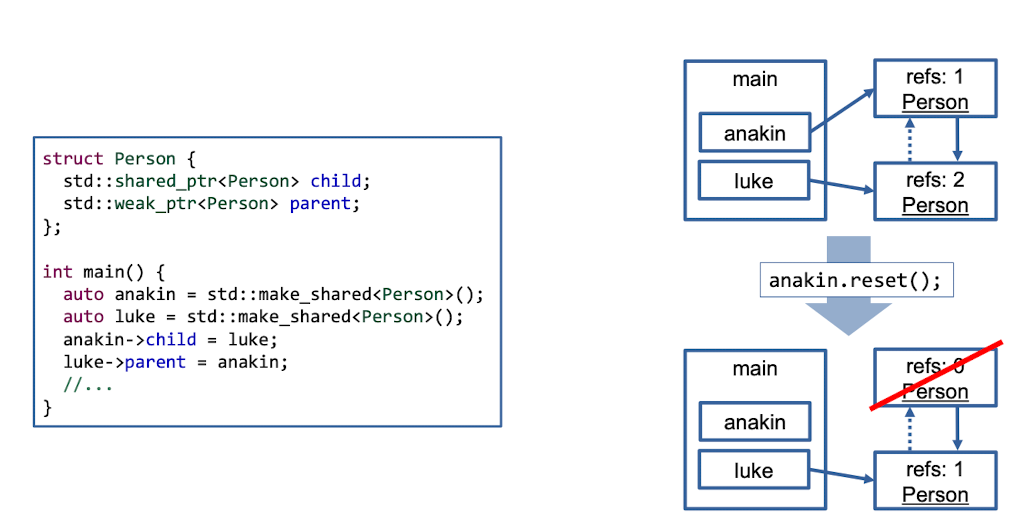
\includegraphics[width=0.75\linewidth]{weakptr}
  \caption{}
\end{figure}
